\section{TJ-Monopix1}
    %%%%%%%%%%%%%%%%%%%%%%%%%%%%%%%%%%%%%%%%
    %%  Slide 1: <TJ-Monopix1>  %%
    %%%%%%%%%%%%%%%%%%%%%%%%%%%%%%%%%%%%%%%%
    \begin{frame}
        \frametitle{TJ-Monopix1}
        Designed by ATLAS collaboration besides LF-Monopix1. 
        Small electrode (), p-type, with process modification in the epi-layer. high resistivity ($>$\SI{1}{k\ohm cm}). Capacity \SI{3}{fF}. ALPIDE like FE.

        \begin{columns}
            \column{0.4\textwidth}  
                \begin{table}
                    \tiny
                    \begin{tabular}{| c |c |}
                    \hline
                    Parameter & Value\\
                    \hline
                    \hline
                    Matrix size &  1$\times$2\si{cm\squared}\\
                    Pixel size & 36 $\times$ 40 \si{\um\squared}\\
                    Depth & \SI{25}{\um}\\
                    Electrode size & \SI{2}{\um}\\
                    BCID & \SI{40}{MHz} \\
                    ToT-bit & 6 \\
                    Power consumption & $\sim$ 120 \si{mW/cm\squared}\\    
                    \hline
                    \end{tabular}
                \end{table}
            \column{0.6\textwidth}  
            Because of a reset element made with PMOS, the discharge of the preamplifier is costant, then the ToT is correlated with the pulse amplitude 
        \end{columns}
    \end{frame} 

    %%%%%%%%%%%%%%%%%%%%%%%%%%%%%%%%%%%%%%%%
    %%  Slide 1: <TJ-Monopix1>  %%
    %%%%%%%%%%%%%%%%%%%%%%%%%%%%%%%%%%%%%%%%
    \begin{frame}
        \frametitle{TJ-Monopix1}
            \centering
            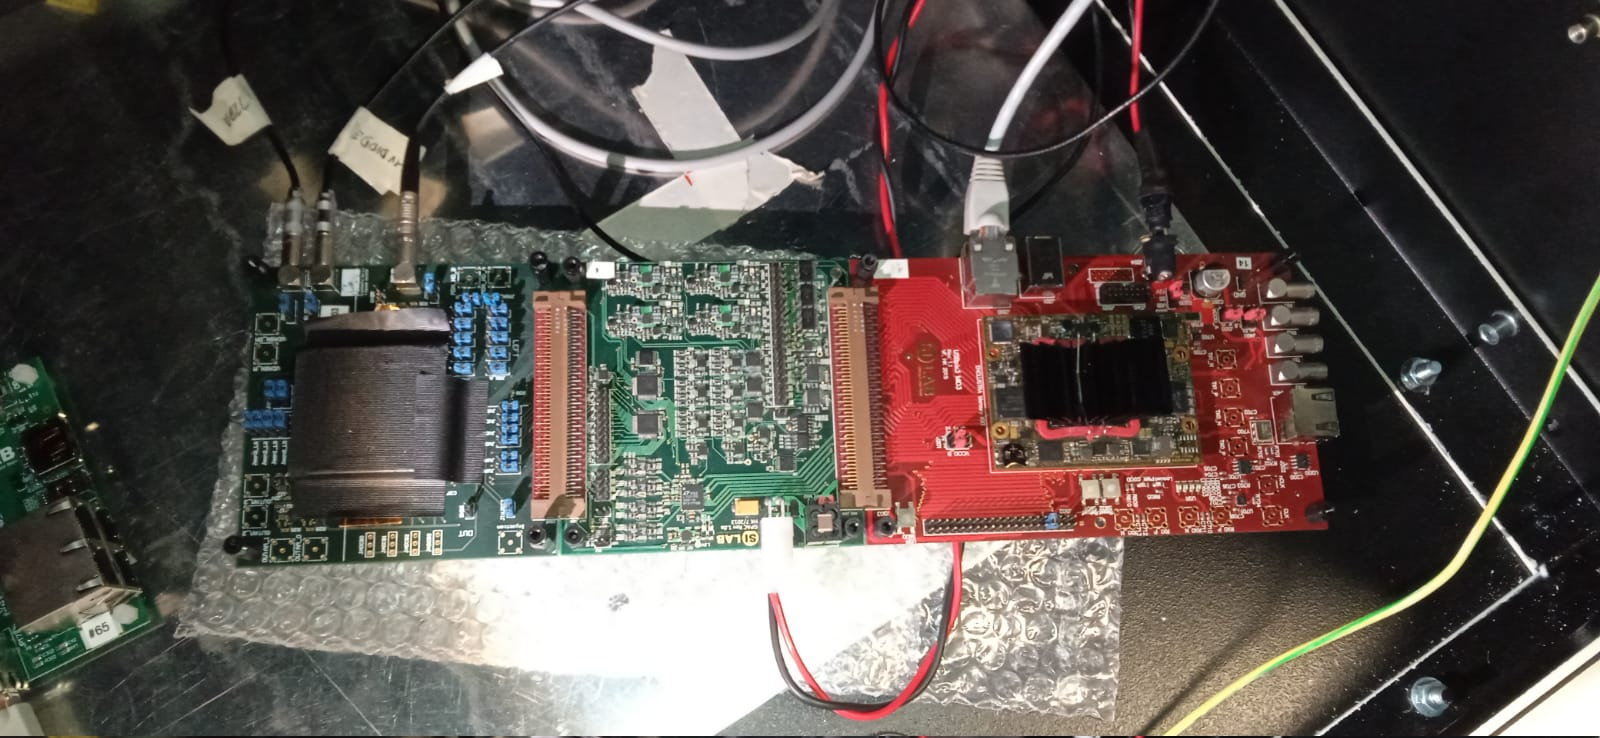
\includegraphics[width=.8\linewidth]{figures/Monopix1/monopix1_front.jpeg}\\
            From left to right DUT, GPAC breakout board and FPGA
    \end{frame} 




    %%%%%%%%%%%%%%%%%%%%%%%%%%%%%%%%%%%%%%%%
    %%  Slide 1: <>  %%
    %%%%%%%%%%%%%%%%%%%%%%%%%%%%%%%%%%%%%%%%
    \begin{frame}
        \frametitle{Front end}
            \textbf{ALPIDE like}
            \begin{figure}[h!]
                \centering
                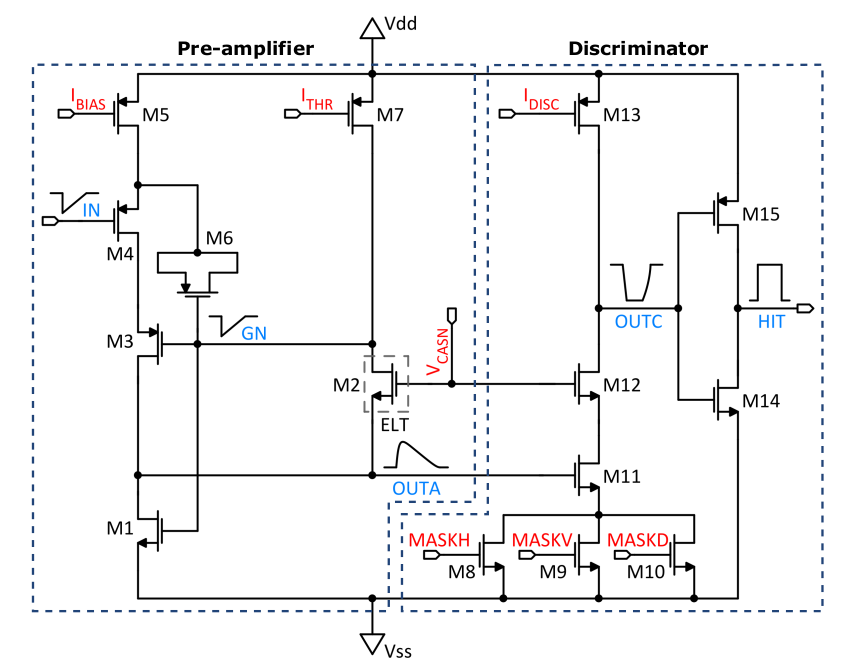
\includegraphics[width=.8\linewidth]{figures/Monopix1/Monopix1_FE_circuit.png}        
            \end{figure}
    \end{frame}     



